\chapter{Návrh a realizácia konštrukcie dvojkolesového robota}

Pred začatím procesu návrhu hardvérového riešenia nášho robota sme postupovali najprv vytvorením zoznamu komponentov, ktoré budú potrebné pre realizáciu robota. Pri návrhu sme brali do úvahy požiadavku na modulárnosť robota. Pod pojmom modulárnosť rozumieme skonštruovanie robota tak, aby jednotlivé jeho časti mohli byť v prípade potreby jednoducho vymenené bez potreby väčších zásahov do konštrukcie. 

Robota sme teda rozdelili do viacerých funkčných celkov a pre každý z týchto celkov vytvorili samostatný zoznam komponentov. Vďaka tomuto postupu sme nielen znížili možnosť výberu nevyhovujúcich súčiastok, ale aj zabezpečili, že naše riešenie bude v prípade potreby škálovateľné a jednotlivé celky bude ľahké pozmeniť alebo doplniť o dodatočné časti. V budúcnosti bude teda možné vymeniť napr. komunikačný modul, bez ovplyvnenia zvyšku robota.

\todo[inline] Precitat znova

\underline{Funkčné celky balansujúceho robota:}
\begin{itemize}
\item napájanie
\item pohon
\item komunikácia
\item senzory
\item riadiaci mikropočítač
\end{itemize}

\section{Zoznam použitých komonentov}

V tejto sekcií opíšeme nami vybrané komponenty, ktoré boli využité pri konštrukcií robota. Zameriame sa hlavne na dôvod voľby daného komponentu, porovnáme špecifikácie použitých komponentov s našimi požiadavkami a zhodnotíme ako dobre sa komponent hodí pre naše použitie.

Na schematickom znázornení nižšie je v blokovej schéme zachytené očakávané rozloženie komponentov, ktoré budú tvoriť robota. Samostatne sme zvýraznili toky energie t.j. napájanie jednotlivých komponentov a toky dát v systéme. 

\begin{figure}
\centering
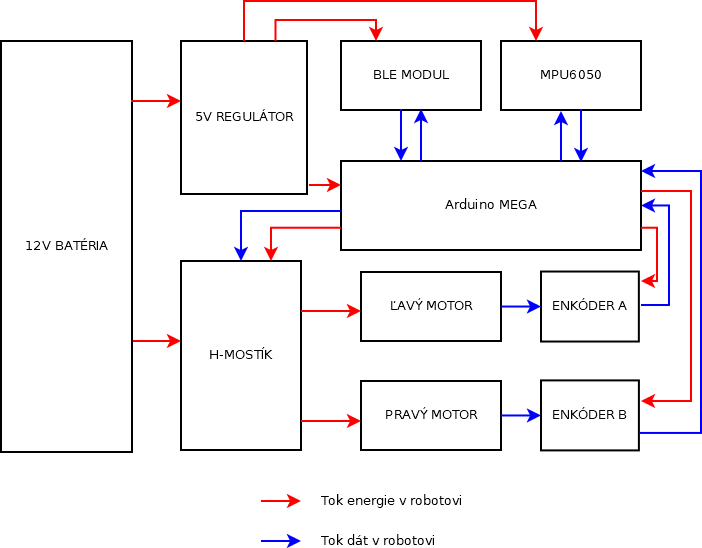
\includegraphics[width=10cm]{tokyDat}
\caption{Schematické zapojenie komponentov}
\label{fig:tokyDat}
\end{figure}

\subsection{Napájanie}
Táto sekcia obsahuje komponenty, ktoré poskytujú vhodné napájanie ostatným častiam robota.
\subsubsection{Batéria}
Pri výbere batérie sme sa snažili nájsť nabíjateľný model, ktorý by nám poskytol pri nízkej hmotnosti čo najvyššiu kapacitu, relatívne vysoký výstupný prúd a napätie pohybujúce sa v rozmedzí 6 V až 12 V, ktoré je dostatočné pre väčšinu bežne dostupných jednosmerných motorov. Rozhodli sme sa teda pre 12V lítium-iónovú (Li-ion) batériu, využívajúcu tri 3,7 V články typu 18650. Kapacita batérie je 3300 mAh, maximálny okamžitý odoberaný prúd 5 A a maximálny pracovný prúd 3A. K nej priložený nabíjací adaptér je schopný dobíjať je prúdom 1 A pri 12,6 V. Spolu s relatívne nízkou hmotnosťou 150g sa teda batéria z \figurename~\ref{fig:bateria} po každej stránke javí ako dobrá voľba. 

\begin{figure}
\centering
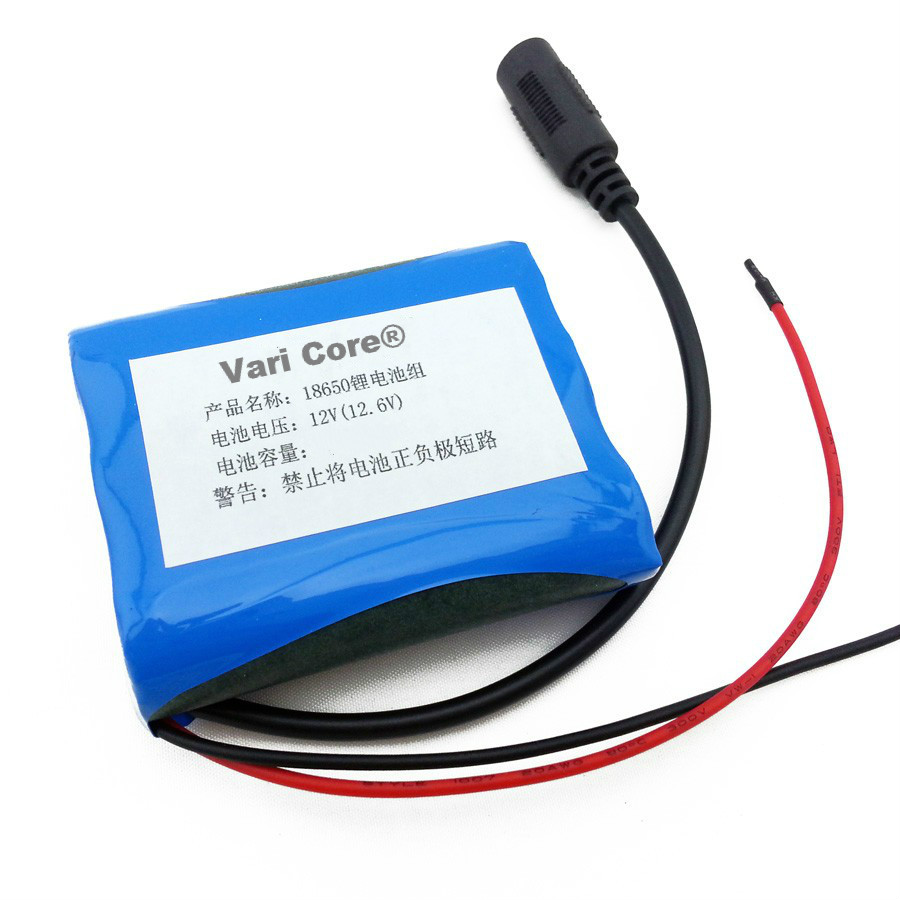
\includegraphics[width = 6cm]{bateria}
\caption{Li-ion batéria}
\label{fig:bateria}
\end{figure}

\subsubsection{Napäťový regulátor pre logické obvody}
Jedným z možných riešení pre napájanie logických odvodov robota, bolo použitie sekundárnej 5 V batérie. Toto riešenie sa ale nejavilo v tomto prípade ako optimálne, keďže druhá batéria by zaberala miesto a vyžadovala si samostatný napájací adaptér. Rozhodli sme sa preto využiť už zabudovanú 12 V batériu napájajúcu motory v kombinácií s napäťovým regulátorom. 

Rozhodovali sme sa medzi rozšíreným integrovaným obvodom L7805CV, ktorý predstavuje 5 V lineárny napäťový regulátor a spínaným napäťovým regulátor LM2596. Vďaka vlastnostiam LM2596 medzi ktoré patrí vysoká účinnosť (až 92\%), malé kolísanie výstupného napätia a možnosť riadenia výstupného napätia od 4 V – 35 V sme sa nakoniec rozhodli použiť ako náš napäťový regulátor \figurename~\ref{fig:napRegulator} práve tento obvod.

\begin{figure}
\centering
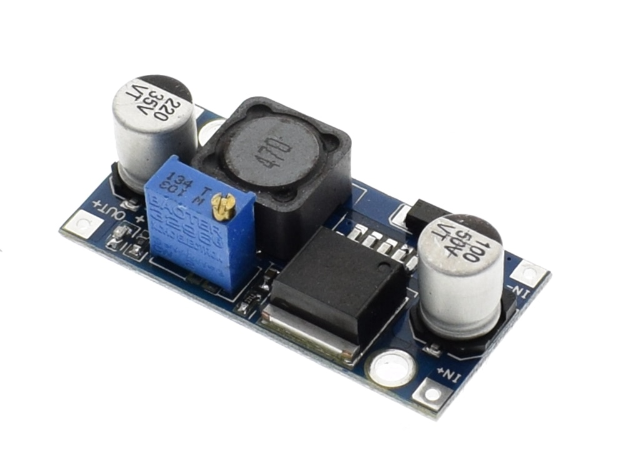
\includegraphics[width=6cm]{napRegulator}
\caption{Spínaný napäťový regulátor kompatibilný s LM2596}
\label{fig:napRegulator}
\end{figure}

\subsection{Pohon}
Pre samotný pohyb robota je potrebné správne zvoliť vhodný typ motora a obvodu, ktorý bude môcť podľa pokynov mikropočítača dané motory ovládať. V našom prípade sme vyberali ako motory, ktoré budú pohánať kolesá robota, tak aj servo motor umožňujúci robotovi reagovať aj na pohyb po naklonených plošinách.

\subsubsection{Motory}
V prípade motorov sme mali na výber z viacerých možností, pričom hlavným kritériom bolo, že sa musí jednať o motory jednosmerné. Aj tak sme ale mohli voliť medzi bezkomutátorovým, krokovým a motorom s permanentnými magnetmi. Po úvahe a prieskume bežne dostupných motorov sme sa rozhodli pre klasický motor s permanentnými magnetmi využívajúci komutátor. Tento motor má niekoľko nevýhod ako sú napríklad malá presnosť v porovnaní s krokovým motorom a menší moment spolu s rýchlejším opotrebením v porovnaní s motorom bez komutátora. Napriek týmto nevýhodám sú tieto motory ale vhodné pre naše účely lebo sú lacné, jednoduché na ovládanie a dostupné v mnohých konfiguráciách. 

Po zvážení sme sa rozhodli pre 12 V motory typu GM25-370CA, s integrovanou prevodovkou 1:21 a zabudovanými dvojkanálovými enkodérmi, ktoré nám umožnia odometrickým meraním sledovať zmenu pozície kolies napojených na motor. Dokumentácia uvádza max. rýchlosť nezaťaženého motora ako 280 rpm (otáčok za minútu), my sme ale namerali skutočnú max. rýchlosť len 220 rpm. Výhodou týchto motorov je, že je možné ich dostať v konfigurácií priamo určenej pre robotické platformy podobné našej spolu s kolesami a kovovým podvozkom. 

\todo [inline] Doplnit tabulku

\begin{figure}
\centering
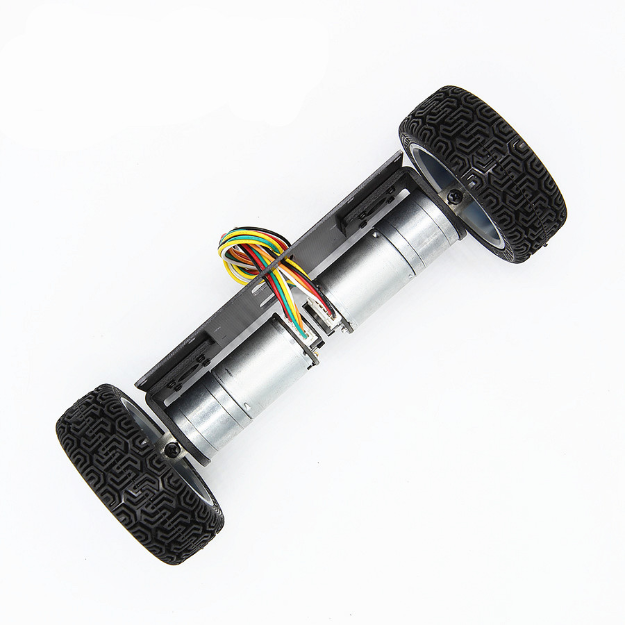
\includegraphics[width=6cm]{motorPlatforma}
\caption{Platforma s motormi}
\label{fig:motorPlatforma}
\end{figure}

\subsubsection{H-mostík}
Keďže mikropočítač nie je bez externej elektroniky schopný sám dodávať do motora potrebný výkon je potrebné spolu s ním použiť tzv. H – mostík. Ten predstavuje principiálne iba štyri elektricky ovládané spínače (viď. príloha X), ktoré podľa svojej konfigurácie menia smer toku prúdu motorom - teda smer otáčania motora. Naše požiadavky na H-mostík boli: vysoká účinnosť, jednoduché prepojenie s mikropočítačom, galvanicky oddelené vstupy mikropočítača a  schopnosť dodať nám vybraným motorom dostatočný výkon (výrobca uvádza maximálny dober 1,5 A na motor). 

Našou voľbou bol dvojitý H-mostík kompatibilný s integrovaným obvodom L298, ktorý spĺňa všetky naše požiadavky a je schopný dlhodobo dodávať do motorov až 7A pri napätí 12V. Tento obvod je možné prepojiť s mikropočítačom pomocou šiestich vstupov, pričom štyri slúžia na výber konfigurácie spínačov a dva prijímajú PWM signál, ovládajúci pripojenie batérie na vstup motorov. Je teda možné jednoducho meniť striedu jednotlivých motorov a tým aj ich rýchlosť. Pre svoju správnu činnosť vyžaduje tento H-mostík napájanie 5 V, to nám poskytne nami použitý napäťový regulátor.  

\begin{figure}
\centering
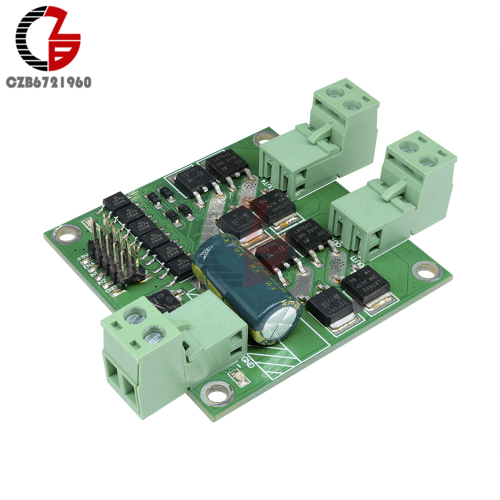
\includegraphics[width=6cm]{hMostik}
\caption{H-mostík komaptibilný s L298}
\label{fig:hMostik}
\end{figure}

\subsubsection{Servo motor}
Jednou z dodatočným požiadaviek na nášho balansujúceho robota bolo, aby sa šasi robota mohlo pohybovať do strán nezávisle od platformy s kolesami. Táto funkcionalita nám v praxi poskytne vyššiu kontrolu nad robotom v zatáčkach, na naklonených plošinách a do určitej miery zníži pravdepodobnosť pádu v prípade pôsobenia silou na bočnú časť robota.

Za optimálne riešenie sme považovali jednoduché servo HJ S3315D určené prevažne na modelárske účely. Toto servo dodatočne taktiež spojí platformu s kolesami a šasi robota, ktorým bude takto možné v prípade potreby hýbať o presne určené uhly. V takejto konfigurácií  obmedzenie pohybu serva v rozmedzí -90º až 90º nepredstavuje problém.

\todo [inline] Zisti ci je to spravny model

\begin{figure}
\centering
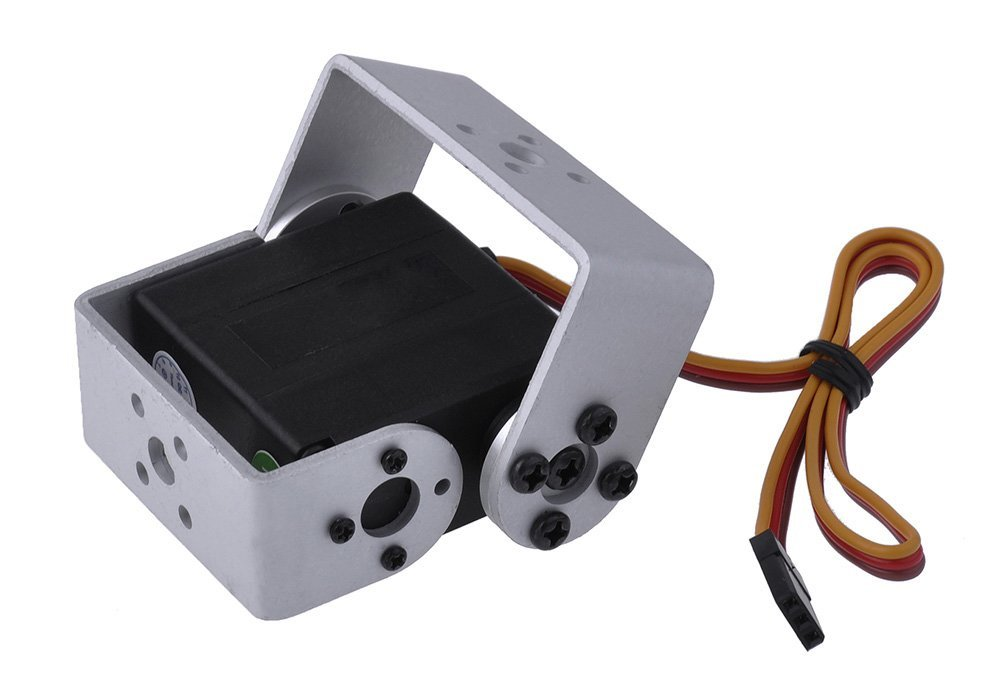
\includegraphics[width=8cm]{servoMotor}
\caption{Servo motor HJ S3315D}
\label{fig:servoMotor}
\end{figure}

\subsection{Komunikácia - Bluetooth modul}
Okrem samotného balansovania na mieste musí byť tiež operátor schopný robota na diaľku riadiť tak aby bol tento schopný pohybovať sa v priestore podľa pokynov. Taktiež je nutné aby bol robot v prípade požiadania operátora schopný poskytnúť základné informácie o svojom stave, napr. úroveň nabitia batérie, priemernú rýchlosť pohybu v určitom časovom intervale, okamžitý uhol náklonu, teplota prostredia… Tieto informácie musí byť robot schopný poskytnúť s čo najmenším oneskorením, bezdrôtovo a minimálne na vzdialenosť 20 metrov.  

Rozhodli sme sa použiť Bluetooth vysielač/prijímač HM-05. Tento modul sa vyznačuje nízkou spotrebou max. 235 $\mu A$, min. $0.4\mu A$ a je schopný ako prijímať tak aj odosielať dáta pomocou rozhrania štandardného rozhrania UART (Universal Asynchronous Reciever-Transmitter). 

Využitím tohoto modulu ako v robotovi tak aj v ovládači, ktorým ho budeme ovládať zabezpečíme ako možnosť odosielať jednoduché povely na riadenie robota, tak aj prijímať komplexné dáta o jeho aktuálnom stave.

\begin{figure}
\centering
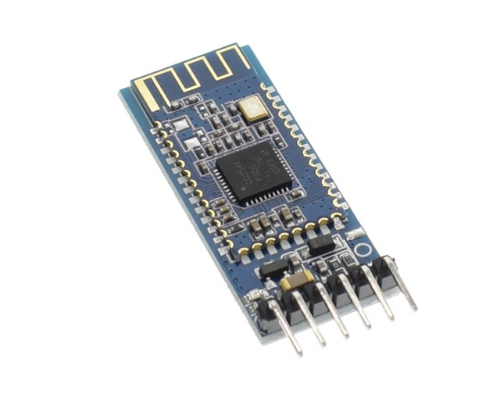
\includegraphics[width=8cm]{bluetoothModul}
\caption{HC05-Bluetooth modul}
\label{fig:bluetoothModul}
\end{figure}

\subsection{Senzory}
Pod senzormi rozumieme všetky časti robota, ktoré mu umožňujú získavať informácie o jeho okolitom prostredí. Pre naše účely je nevyhnutné presne merať uhol náklonu robota, rýchlosť pohybu motorov a prúd do motorov

\subsubsection{MPU 6050}
Pre úspešné balansovanie robota je potrebná relatívne vysoká presnosť merania uhla náklonu robota. Ak by sme postupovali využitím akcelerometra, prístroja určujúceho uhol náklonu podľa pôsobenia gravitačného zrýchlenia, nebolo by toto meranie dosť presné, keďže pri rýchlych zmenách polohy by nebol akcelerometer schopný reagovať dosť rýchlo. Býhodou akcelerometického merania je však veľmi vysoká presnosť merania v ustálenom stave. Naproti tomu gyroskop, prístroj merajúci uhlovú rýchlosť, by po integrovaní nameraných hodnôt bol schopný určiť zmenu uhla za časový okamih dt – teda aj novú polohu v prípade, že poznáme tu predchádzajúcu. Problémom použitia gyroskopu ale je, že aj tá najmenšia chyba pri každom meraní a integrovaní sa započíta do výsledku a po niekoľkých stovkách meraní je už chyba merania uhla značná – tomuto javu sa hovorí gyroskopický drift. 

Riešenie problému merania uhla v pohybujúceho sa robota predstavuje kombinácia nameraných hodnôt z akcelerometra a gyroskopu, pomocou komplementárneho filtra. Na toto využite sa hodí modul MPU 6050, ktorý v sebe kombinuje trojosový akcelerometer a gyroskop. Modul je schopný komunikovať s mikropočítačom pomocou rozhrania I2C maximálnou rýchlosťou 400kHz a obsahuje taktiež integrovaný teplomer a DMP (Digital Motion Processor).Ten je schopný priamo uskutočniť analýzu nameraných dát, čím sa znížia požiadavky na výpočtový čas mikropočítača.

\begin{figure}
\centering
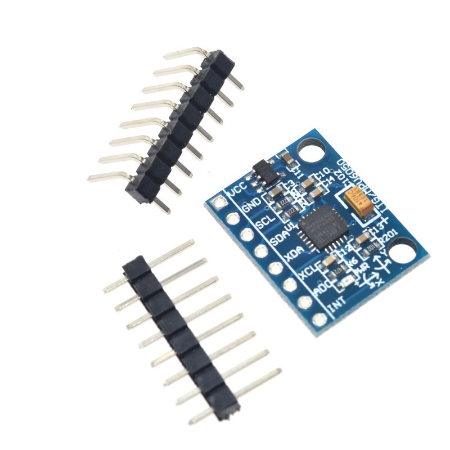
\includegraphics[width=8cm]{MPU}
\caption{MPU6050}
\label{fig:MPU}
\end{figure}

\subsection{Riadiaci počítač - Arduino MEGA}
Vďaka skúsenostiam s programovaním mikropočítačov spoločnosti Microchip-Atmel sme sa pri výbere mikropočítača rozhodovali medzi mikropočítačmi rodiny ATMEGA. Do úvahy spadali hlavne ATMEGA328P a ATMEGA2560, ktorých výpočtové možnosti a zabudované periférie postačovali našim požiadavkám. Jednou zo zvažovaných možností bolo navrhnutie a skonštruovanie obvodu so zabudovaným mikropočítačom, ktorý by priamo zodpovedal požiadavkám našej aplikácie. Toto riešenie sme ale nakoniec po úvahe zavrhli, keďže by bolo časovo náročné a nespadalo by do koncepcie modularity – takto navrhnutý obvod by v prípade poruchy bol náročný na nahradenie a bolo by veľmi náročné upraviť ho pri zmene požiadaviek na robota.

Rozhodli sme sa teda využiť rozšírenú, otvorenú, vývojovú platformu Arduino, ktorá vo všeobecnosti slúži na vývoj prototypov a testovanie kódu. Našou voľbou bolo Arduino MEGA \figurename~\ref{fig:arduinoMega}, využívajúce mikropočítač ATMEGA2560. Táto vývojová doska má zabudovaný programovací port USB typu B (ktorý sme zamenili na micro USB), napäťový regulátor na 5V a 3.3V, 16 MHz oscilátor (zdroj hodinového signálu pre mikropočítač) a na rozdiel od lacnejšieho Arduino Uno má až 53 GPIO (General Purpose Input Output) pinov, 16 pinov podporujúcich ADC (prevod analógového signálu na jeho digitálnu reprezentáciu) a 6 pinov podporujúcich niekoľko režimov prerušení.

Samotný mikropočítač má viacero časovačov, ktoré umožňujú napr. merať časové intervaly a generovať PWM signál, ale taktiež 4 páry RX, TX pinov slúžiacich na komunikáciu pomocou UART protokolu. Ako ďalšie možnosti komunikácie je možné využiť aj I2C a SPI protokoly. Programovanie dosky Arduino MEGA je možné cez USB rozhranie napr. pomocou programu ArduinoIDE, AtmelStudio alebo Eclipse. Našou voľbou bolo využitie všestranného editora Eclipse, v kombinácií s pluginom umožňujúcim jednoduchú prácu s mnohými produktami Microchip-Atmel.

\begin{figure}
\centering
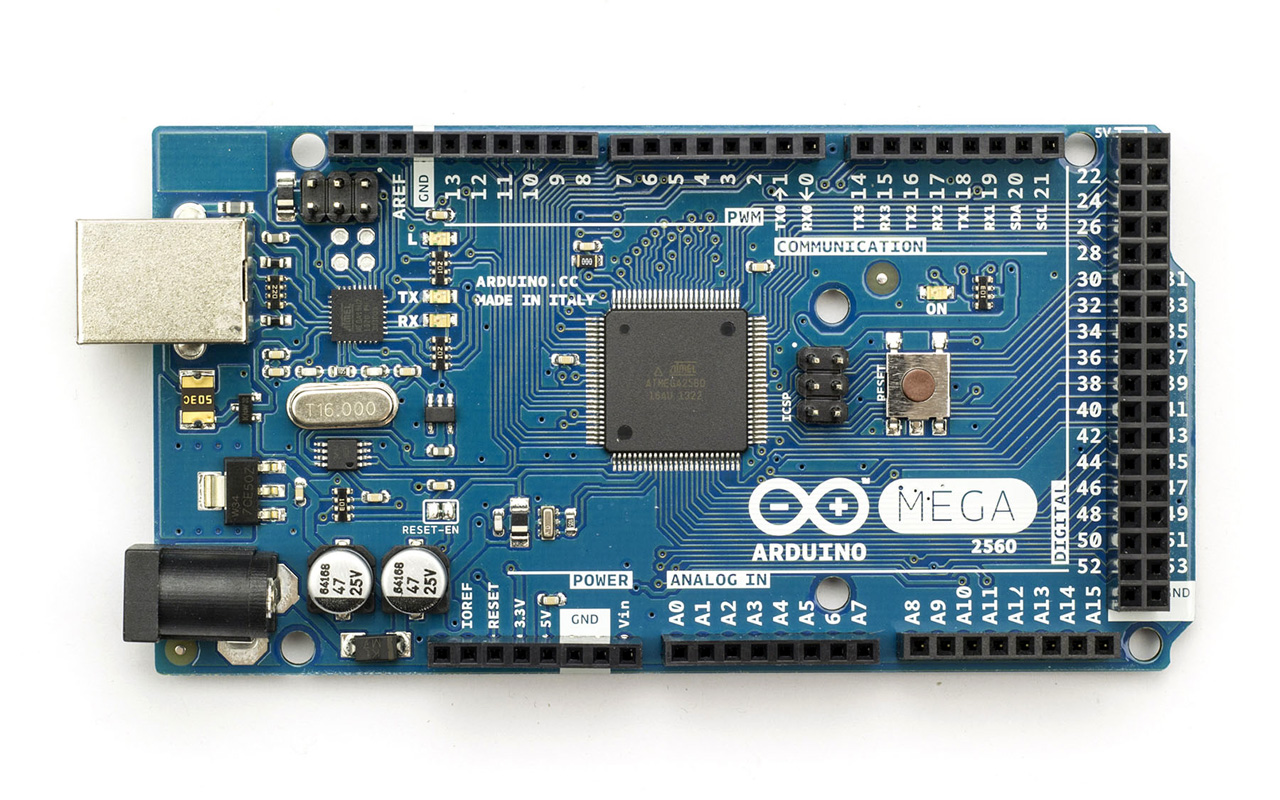
\includegraphics[width=8cm]{arduinoMega}
\caption{Arduino MEGA}
\label{fig:arduinoMega}
\end{figure}

\section{Návrh a výroba šasi robota}
Pri výrobe šasi robota sme sa rozhodli použiť technológiu 3D tlače. S jej použitím sme boli schopný vytvoriť pevné a ľahké šasi, ktoré presne zodpovedalo našim požiadavkám. Pred samotnou tlačou sme ale museli navrhnúť model v CAD programe, tak, aby bolo nielen jednoduché ho vytlačiť, ale aj aby bolo schopné odolať nárazom a ochrániť tak elektroniku vnútri. Pri návrhu sme použili software Fusion 360, ktorý je pre študentov dostupný zdarma na stránke firmy Autodesk (\href{https://www.autodesk.com/products/fusion-360/overview}).

Program Fusion 360 podporuje ako návrh a export modelov do viacerých bežne používaných formátov, tak aj analýzu vlastností modelu, simuláciu jeho správania pri záťaži, nástroje na vizualizáciu, animáciu a mnoho ďalších užitočných funkcií.

\begin{figure}
\centering
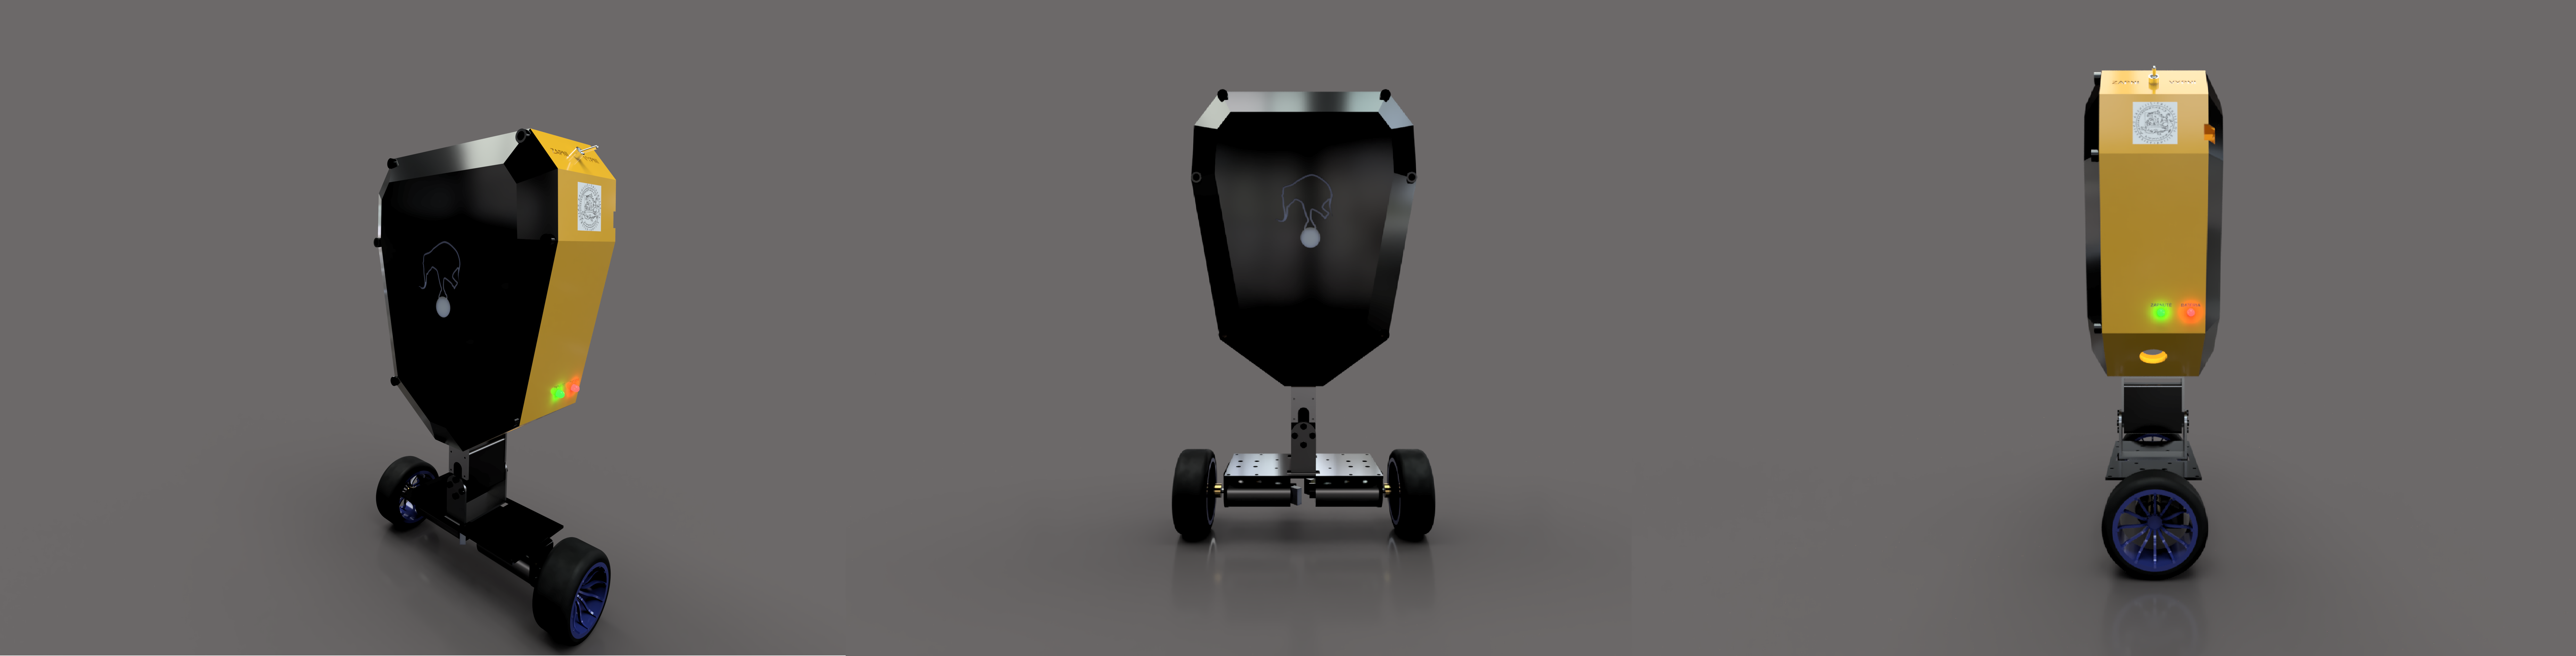
\includegraphics[width=12cm]{robotVizu}
\caption{Vizualizácia robota v programe Fusion 360}
\label{fig:robotVizu}
\end{figure}

Nami vytvorené šasi \figurename~\ref{fig:robotVizu} sa skladá z dvoch častí a to veka a miskovitého tela, v ktorom sú uložené komponenty. Po naštudovaní prác, ktoré už boli na tému návrhu dvojkolesového balansujúceho robota napísané sme zvolili pre celé šasi klinovitý tvar, s úzkou podstavou a širokých vrchom. Tento tvar nám umožní jednoduché napojenie servomotora na spodnú časť robota a osadenie batérie blízko k hornej časti robota. V takejto pozícií batérie dosiahneme relatívne vysoko umiestnené ťažisko, čo následne zjednoduší stabilizovanie robota. Šasi taktiež obsahuje otvory na kabeláž od motorov, dve status LED diódy, spínač napájania a prístup k portu micro USB, vďaka ktorému je možné robota programovať bez nutnosti demontáže veka.

Samotná tlač prebehla po vytvorení .gcode súboru v nástroji Cura na tlačiarni Creality CR-10s. Na tlač bol použitý materiál PLA (Polyactic Acid), ktorý sa vyznačuje nízkou tepelnou rozťažnosťou pri chladnutí, nízkou cenou a jednoduchou tlačou. 

\begin{figure}
\centering
\includegraphics[width=8cm]{robotOutsideFoto}
\caption{Balansujúci robot s osadenými motormi}
\label{fig:robotOutsideFoto}
\end{figure}

Samotná tlač trvala približne 50 hodín, kvôli požiadavke na relatívne vysokú presnosť (a teda malú výšku jednotlivých vrstiev) a spotrebovalo sa pri nej približne 0,5 kg filamentu PLA. Po vytlačení, osadení komponentov a nalakovaní sa nami vytvorený model \figurename~\ref{fig:robotOutsideFoto} výzorom blížil k jeho počítačovo vygenerovanej podobe \figurename~\ref{fig:robotVizu}. Po kontrole môžeme tiež konštatovať, že vnútorné a vonkajšie rozmery oboch dielov presne zodpovedali nášmu návrhu.

Pri tlači sa vyskytli menšie chyby, ktoré spôsobili artefakty na veku robota v podobe pruhov spôsobených krycou páskou na podstave tlačiarne. Ako problematické sa ukázalo taktiež vytlačenie tela, na ktorého povrchu boli po vytlačení viditeľné vady v podobe nezaplnených miest a príliš zaoblených hrán. Tie mohli byť spôsobené nesprávnym nastavením parametrov v programe Cura, privysokou teplotou vyhrievanej podstavy tlačiarne alebo príliš priľnavou podstavou. 

Výsledné výtlačky boli ale použiteľné, keďže vyššie opísané vady boli čisto estetického charakteru. Ako závažnejším problémom sa ukázala realizácia kabeláže. Napriek dostatku miesta bolo po zapojení všetkých komponentov náročné sa v kabeláži vyznať, čo by mohlo spôsobiť problémy pri dodatočnej údržbe. Taktiež, keďže niektoré súčasti zapojenia nebolo možné realizovať na doske Arduino, keďže by si vyžadovali použitie dodatočných komponentov, boli by sme na ich realizáciu nútení použiť dosku plošných spojov, čo by následne ešte zhoršilo prehľadnosť kabeláže.

\begin{figure}
\centering
\includegraphics[width=8cm]{robotInsideFoto}
\caption{Osadenie komponentov}
\label{fig:robotOutsideFoto}
\end{figure}

Ako problém z neprehľadnosťou kabeláže tak aj s ďalšími potrebnými komponentami sme sa rozhodli adresovať návrhom a konštrukciou tzv. shieldu - čiže dosky plošných spojov, ktorá svojim vyhotovením bude predstavovať nadstavbu Arduina. Tento shield sa pripojí na výstupy Arduina a bude obsahovať označené terminály na pripojenie všetkých komponentov.

Návrh tejto dosky plošných spojov sme uskutočnili v bezplatnej verzií nástroja Eagle. Tá umožňuje návrh elektrických schém aj PCB (Printed Circuit Board) a generovanie gerber súborov, ktoré obsahujú informácie pre výrobcu. Ukážka takto vytvorenej dosky je v prílohe , pričom pri jej tvorbe sme vychádzali zo schémy na \figurename~\ref{fig:schemaShield}. 

Zo schémy je zjavné, že nami vytvorený obvod obsahuje okrem vstupno/výstupných terminálov aj dodatočnú ochranu vstupov proti prepätiu. Táto je realizovaná formou zenerových diód s hodnotou prierazného napätia 5 V, zapojených v závernom smere. Napriek tomu, že mikropočítač ATmega 2560 obsahuje zabudované diódy, ktoré vedia vstupy ochrániť proti krátkodobému prepätiu, externé zenerove diódy prejdú do vodivého stavu skôr a zabránia tak prípadnému poškodeniu mikropočítača prepätím. 

Medzi ďalšie ochranné prvky, ktoré sme implementovali patrí, voči kladnému pólu batérie, sériovo zapojená schottkyho dióda, ktorá zabráni poškodeniu komponentov v prípade nesprávneho pripojenia batérie. Podobným spôsobom zapojená tavná poistka ochráni batériu pred možným skratom v obvode.  Keďže bluetooth modul, ktorý sme zvolili pre realizáciu komunikácie, pracuje s logickými úrovňami od 0 V do 3,3 V, ale Arduino výstupy pracujú s 5 V pripojili sme RX vstup modulu k mikropočítaču cez napäťový delič. 

Doska plošných spojov obsahuje aj dva potenciometre, tri spínače a reproduktor. Potenciometre a spínače budú v prípade potreby slúžiť na jemnú kalibráciu alebo manuálne zadávanie jednoduchých povelov. Reproduktor so zabudovaným oscilačným obvodom slúži ako hlásič, napr. v prípade prebiehajúcej kalibrácie.

\todo [inline] {Hodit obr. do prilohy}
\begin{sidewaysfigure}[p]
\centering
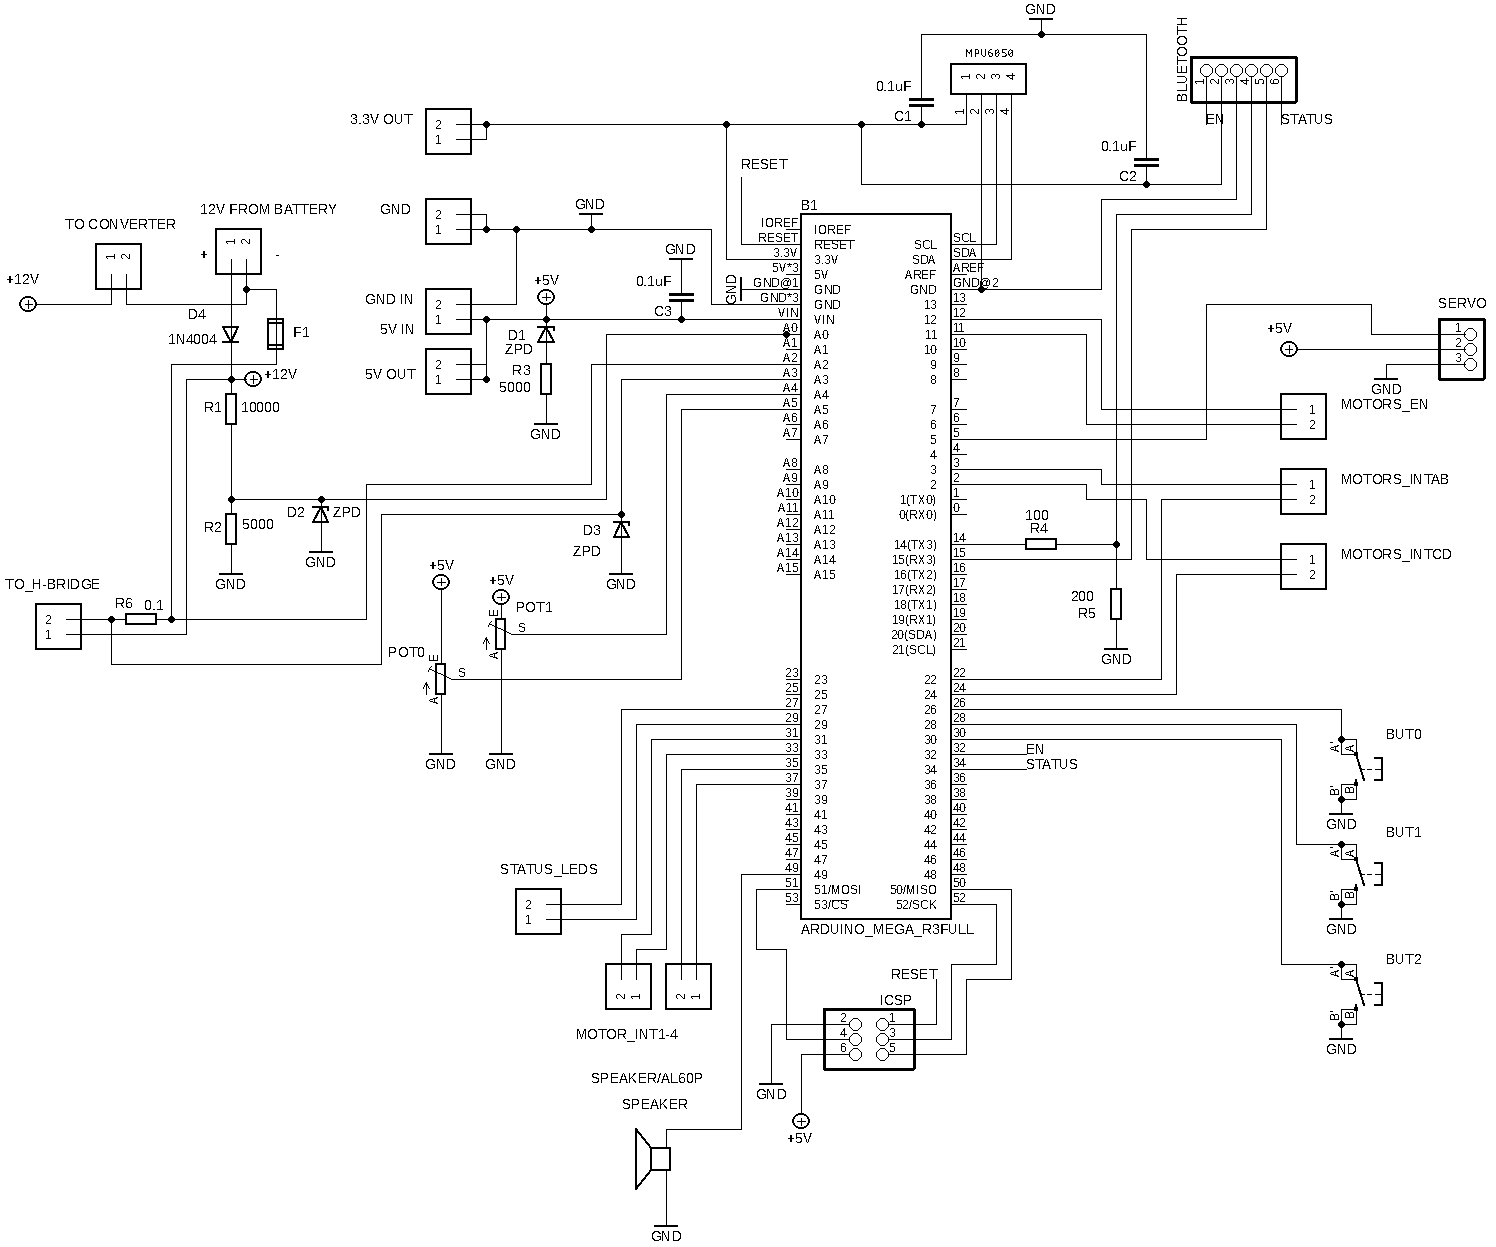
\includegraphics[width=23cm]{schemaShield}
\caption{Schéma shieldu pre Arduino}
\label{fig:schemaShield} 
\end{sidewaysfigure}

\section{Návrh a výroba ovládača robota}

Pri návrhu ovládača robota sme postupovali obdobným spôsobom ako pri návrhu šasi. Rovnako ako pri šasi aj tu bol na návrh ovládača použitý nástroj Fusion 360 a technológia 3D tlače. Takto navrhnutý ovládač obsahuje dvojosový analógový joystick, ktorý riadi pohyb robota a umožňuje používateľovi pohyb v menu nastavení. Informácie získava používateľ zo zabudovaného 1,8 palcového farebného TFT displeja. Orientáciu v menu zjednodušujú dve zabudované tlačidlá.

\begin{figure}
\centering
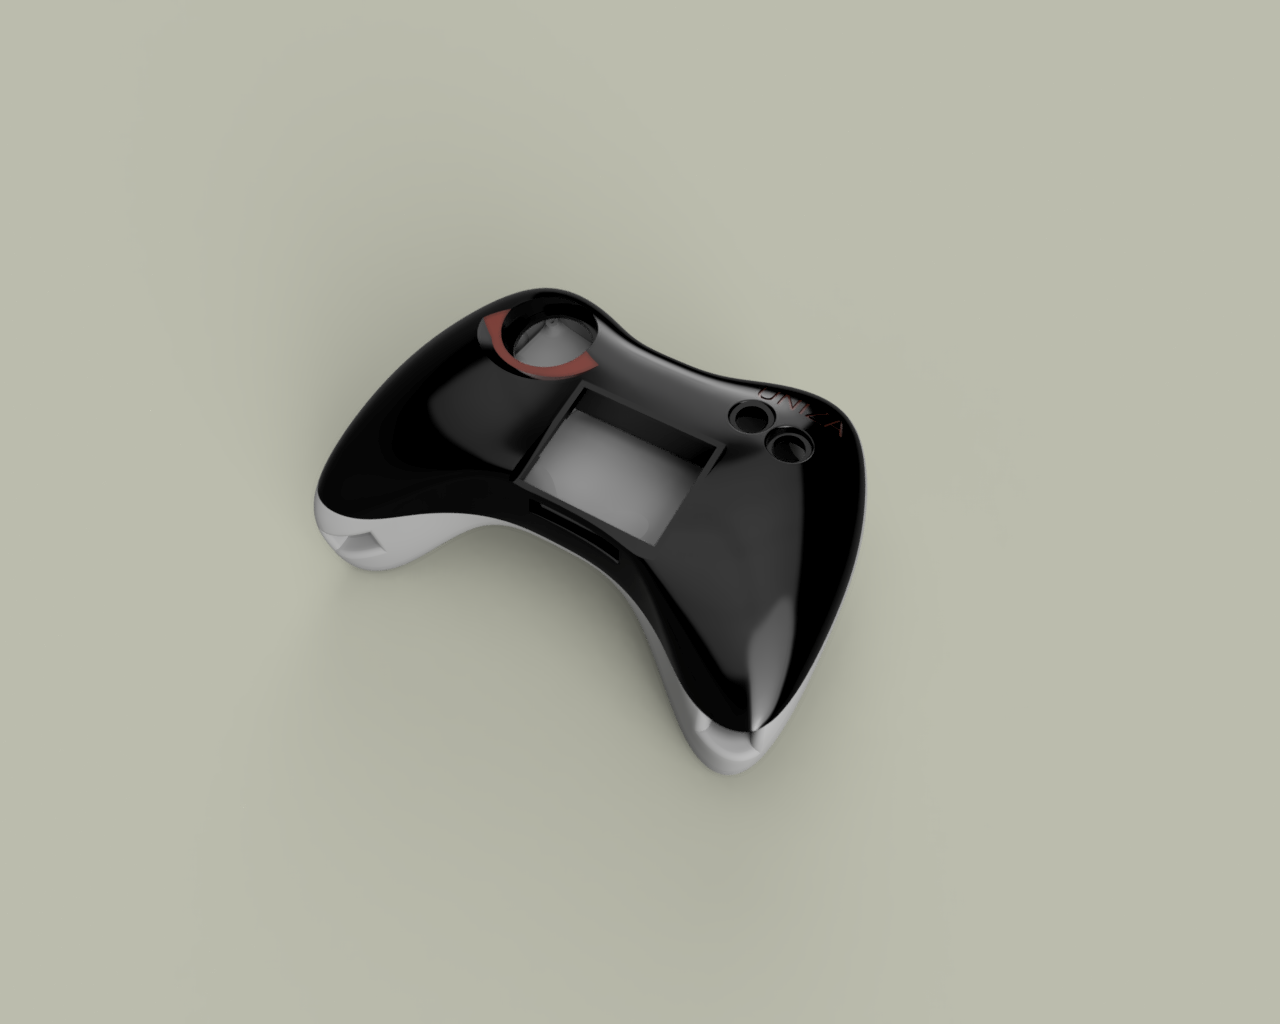
\includegraphics[width=8cm]{kontrolerVizu}
\caption{Ovládač balansujúceho robota}
\label{fig:kontrolerVizu}
\end{figure}

Napájanie ovládača je riešené z klasickej 9V batérie, zredukovanej spínaným zdrojom na 5V a na samotnú komunikáciu slúži modul HC-05 spomenutý v prvej časti tejto kapitoly. Okrem vysielania riadiacich príkazov ovládač v periodických intervaloch prijíma od robota dáta o jeho stave, ktoré následne zobrazuje užívateľovi na displeji.
 
Ovládač je schopný zobraziť informácie o uhle náklonu robota, aktuálnej rýchlosti, priemernej rýchlosti, aktuálnych kalibračných hodnotách a stave batérie. Používateľ môže prostredníctvom ovládača dať robotovi pokyn na začatie autokalibrácie, odosielania dát do terminála počítača cez sériový port alebo na vyslanie výstražného zvukového znamenia.

Narozdiel od predchádzajúceho prípadu, kedy sme navrhli okrem šasi taktiež dosku plošných spojov, v prípade ovládača neexistujú požiadavky na nijakú dodatočnú elektroniku a tak táto potreba odpadá. Komponenty budú spojené vnútri ovládača priamo s vývojovou doskou Arduino Nano. Malé rozmery tejto dosky zabezpečia, že rozmery ovládača budú podobné bežne predávaným konzolovým ovládačom. 

Ako problematická sa ukázala spotreba spínaného regulátora napätia, ktorá v bola v prípade nezaťaženého regulátora až 8 mA. Takýto trvalý odber by nami použitú batériu rýchlo zničil, pristúpili sme teda k priradeniu spínača, ktorým bude batériu možné priamo odpojiť keď bude ovládač nepoužívaný.